\documentclass{easychair}

\newcommand{\easychair}{\sf{easychair}}
\newcommand{\miktex}{MiK{\TeX}}
\newcommand{\texniccenter}{{\TeX}nicCenter}
\newcommand{\makefile}{\texttt{Makefile}}

\usepackage[T1]{fontenc}
\usepackage{lmodern}
\usepackage{epsfig}
\usepackage{subfig, syntonly, comment, amsmath, amssymb, cite, graphicx}
\usepackage{nomencl}
\usepackage{amsthm}
\usepackage[utf8]{inputenc}
\usepackage[portuges]{babel}
\usepackage{url}
\usepackage{hyperref}
\usepackage{booktabs}

\begin{document}

\title{Medição da obesidade através de técnicas de mineração de dados e aprendizagem de máquina.}

\titlerunning{ }

\author{Gonçalo Amaro\\
  Universidade de Évora\\
  \url{m56870@alunos.uevora.pt}\\
}

\authorrunning{G. Amaro}

\maketitle

\begin{abstract}
A obesidade é um problema de saúde pública que afeta milhões de pessoas em todo o mundo. A sua medição é feita através do Índice de Massa Corporal (IMC), que é calculado a partir do peso e altura de um indivíduo. No entanto, o IMC não é um indicador perfeito, pois este não têm em conta a idade ou os fatores sociais e ambientais. Neste trabalho, é proposto um modelo de aprendizagem de máquina para prever a obesidade de um indivíduo, com base em dados demográficos e de estilo de vida.
\end{abstract}

\section{Introdução}

\subsection{Contexto e Significado}

Este trabalho tem como objetivo a criação de um modelo de aprendizagem de máquina para prever a obesidade de um indivíduo, com base em dados demográficos e de estilo de vida, estando sempre dentro de um contexto de ser um trabalho para avaliação de uma unidade curricular. Expandido desse contexto tentaremos tambem retirar conclusões sobre a obesidade e a sua relação com os dados demográficos e de estilo de vida, através de análise de agrupamentos e de visualizações.

\subsection{Objetivos do Estudo}

Temos como objetivo a criação de um modelos de categorização de obesidade, dos quais possamos retirar quais os fatores mais importantes para a obesidade, e quais os fatores que mais influenciam a obesidade. Para além disso, pretendemos também retirar conclusões sobre a obesidade e a sua relação com os dados demográficos e de estilo de vida, através de análise de agrupamentos e de visualizações.

\subsection{Resumo da Metodologia}

Para a realização deste trabalho, foi utilizado o conjunto de dados \textit{Obesity Data Set} \cite{obesity}, que contém dados demográficos e de estilo de vida de 2111 indivíduos, e que foi disponibilizado no repositório \textit{Kaggle} \cite{kaggle}. Este conjunto de dados foi pré-processado, e foram criados três modelos de aprendizagem de máquina para prever a obesidade de um indivíduo, sendo estes modelos de Árvore de Decisão, Máquina de Vetores de Suporte (SVM) e Floresta Aleatória. Para além disso, foi também realizada uma análise de agrupamentos, com o objetivo de retirar conclusões sobre a obesidade e a sua relação com os dados demográficos e de estilo de vida.

\section{Revisão da Literatura}
\subsection{Estudos Anteriores sobre Análise da Obesidade}

Foi verificado que existem vários estudos que utilizam técnicas de aprendizagem de máquina para prever a obesidade de um indivíduo, no entanto existem alguns que são mais curiosos e originais. Foram escolhidos como exemplo dois estudos, um que utiliza técnicas de aprendizagem de máquina para prever a obesidade de um indivíduo, e outro que utiliza técnicas de aprendizagem de máquina para prever a obesidade de um indivíduo, mas que utiliza também a Internet das Coisas (IoT) para recolher os dados.

\begin{itemize}
  \item \textbf{Estimation of obesity levels based on computational intelligence} \cite{estimation} - Neste estudo, foi utilizado um conjunto de dados com 2111 indivíduos, e foram criados três modelos de aprendizagem de máquina para prever a obesidade de um indivíduo. Muito semelhante ao este trabalho, onde foi inspirado, no entanto, neste estudo, foram utilizados como modelos de aprendizagem de máquina o K-Means, Decision Trees (DT), e Support Vector Machines (SVM).
  \item \textbf{IoT Framework for a Decision-Making System of Obesity and Overweight Extrapolation among Children, Youths, and Adults} \cite{iot} - Semelhante ao anterior mas com o twist de ser adaptado para um possível sistema de IoT, onde os dados são recolhidos através de sensores, e são utilizados para meios estrategicos de saúde pública.
\end{itemize}

\section{Dados e Metodologia}

Nesta secção, é apresentada a metodologia utilizada para a realização deste trabalho, bem como a descrição do conjunto de dados utilizado, as técnicas de pré-processamento, as estatísticas resumidas, e a descrição dos modelos de aprendizagem de máquina e de análise de agrupamentos.

\subsubsection{Fonte dos Dados}

Este trabalho utiliza o conjunto de dados \textit{Obesity Data Set} \cite{obesity}, que contém dados demográficos e de estilo de vida de 2111 indivíduos, e que foi disponibilizado no repositório \textit{Kaggle} \cite{kaggle}. Este conjunto de dados já vem pré-processado, no entanto, foi necessário realizar mais pré-processamento para que os modelos de aprendizagem de máquina funcionassem corretamente.

\subsection{Descrição do Conjunto de Dados}

Este conjunto de dados contém 17 atributos, sendo 8 atributos demográficos e 9 atributos de estilo de vida, e um atributo de classe, que é a obesidade. Os atributos demográficos são: idade, sexo, altura, peso, índice de massa corporal (IMC), índice de obesidade (NObeyesdad), tipo de trabalho e nível de atividade física. Os atributos de estilo de vida são: consumo de álcool, fuma, horas de sono, tempo de uso de dispositivos eletrónicos, atividade física, consumo de vegetais, consumo de carne, consumo de refrigerantes e consumo de água. O atributo de classe, obesidade, é dividido em 7 classes, sendo estas: Insuficiente, Normal, Sobrepeso Nível I, Sobrepeso Nível II, Obesidade Tipo I, Obesidade Tipo II e Obesidade Tipo III.

Como podemos ver na tabela de baixo, o conjunto de dados contém 2111 instâncias, e não contém valores em falta. Os atributos demográficos são todos numéricos, e os atributos de estilo de vida são todos categóricos. O atributo de classe, obesidade, é categórico, e contém 7 classes. A pré-analise está disposta na tabela\ref{tab:summary}.

Noto que nem todos os atributos aparecem na tabela sendo que os atributos que não aparecem são os atributos categóricos.

\subsubsection{Principais Atributos}

Como podemos ver na tabela\ref{tab:importance}, os atributos mais importantes para a classificação da obesidade são o peso, a idade, a altura, a frequência de consumo de vegetais, o número de refeições principais, o tempo de uso de dispositivos eletrónicos, o sexo masculino, a frequência de atividade física, o consumo de água e o sexo feminino.

Estes atributos são importantes de formas diferente, as quais carecem de interpretação. Esta pode ser feita através de visualizações, que serão apresentadas na secção de Visualização de Dados.

A descoberta será mais aprofundada na secção de Análise de Agrupamentos.

\subsection{Técnicas de Pré-processamento}

Para a realização deste trabalho, foi necessário realizar pré-processamento ao conjunto de dados, de forma a que os modelos de aprendizagem de máquina funcionassem corretamente. O pré-processamento realizado foi o seguinte:

\begin{itemize}
  \item \textbf{Scaling} - Os atributos numéricos foram escalados, de forma a que os modelos de aprendizagem de máquina funcionassem corretamente.
  \item \textbf{Encoding} - Os atributos categóricos foram codificados para valores numéricos, de forma a que os modelos de aprendizagem de máquina funcionassem corretamente.
\end{itemize}

Qualquer outro pré-processamento foi realizado pelo autor do conjunto de dados. Sendo que nos facilitou o trabalho.

\subsection{Estatísticas Resumidas}

\begin{table}[hbt!]
  \centering
  \begin{tabular}{l c c c c c c c c}
  \toprule
  Feature & Count & Mean & Std & Min & 25\% & 50\% & 75\% & Max \\
  \midrule
  Age & 2111 & 24.31 & 6.35 & 14.00 & 19.95 & 22.78 & 26.00 & 61.00 \\
  Height & 2111 & 1.70 & 0.09 & 1.45 & 1.63 & 1.70 & 1.77 & 1.98 \\
  Weight & 2111 & 86.59 & 26.19 & 39.00 & 65.47 & 83.00 & 107.43 & 173.00 \\
  FCVC & 2111 & 2.42 & 0.53 & 1.00 & 2.00 & 2.39 & 3.00 & 3.00 \\
  NCP & 2111 & 2.69 & 0.78 & 1.00 & 2.66 & 3.00 & 3.00 & 4.00 \\
  CH2O & 2111 & 2.01 & 0.61 & 1.00 & 1.58 & 2.00 & 2.48 & 3.00 \\
  FAF & 2111 & 1.01 & 0.85 & 0.00 & 0.12 & 1.00 & 1.67 & 3.00 \\
  TUE & 2111 & 0.66 & 0.61 & 0.00 & 0.00 & 0.63 & 1.00 & 2.00 \\
  \bottomrule
  \end{tabular}
  \caption{Sumário das Estatísticas do Conjunto de Dados}
  \label{tab:summary}
\end{table}

Como podemos ver na tabela\ref{tab:summary}, o conjunto de dados é bastante variado Este em termos de equilibrio é bastante bom, sendo que não existem valores em falta, e os valores estão bem distribuidos.

\section{Desenvolvimento e Análise do Modelo}

Aqui chegamos ao ponto de desenvolvimento do modelo, onde iremos apresentar os modelos de aprendizagem de máquina e de análise de agrupamentos, bem como as suas configurações e justificações. Sendo este um problema de classificação, foram criados três modelos de aprendizagem de máquina para prever a obesidade de um indivíduo, sendo estes modelos de Árvore de Decisão, Máquina de Vetores de Suporte (SVM) e Floresta Aleatória. Para além disso, foi também realizada uma análise de agrupamentos, mas isso será abordado mais à frente.

A razão pela qual foram escolhidos estes modelos de aprendizagem de máquina, foi porque estes são modelos de aprendizagem de máquina bastante simples, e que são bastante utilizados para problemas de classificação. Para além disso, estes modelos de aprendizagem de máquina são bastante interpretáveis, o que é importante para este trabalho.

A ordem de expectativa de desempenho inicial favorecia a Maquina de Vetores de Suporte, seguido da Floresta Aleatória e por fim a Árvore de Decisão, devido sua natureza n-dimensional e a sua capacidade de separar dados linearmente. No entanto, a ordem de expectativa de desempenho final favorecia a Floresta Aleatória, seguido da Arvore de Decisão e por fim a Maquina de Vetores de Suporte.

Os \textit{scores} de validação cruzada foram calculados utilizando a métrica de \textit{accuracy} em primeiro lugar, e depois utilizando a métrica de \textit{precision}, \textit{recall} e \textit{f1-score}. A métrica de \textit{accuracy} foi utilizada para avaliar o desempenho geral do modelo, e as métricas de \textit{precision}, \textit{recall} e \textit{f1-score} foram utilizadas para avaliar o desempenho do modelo para cada classe.

% introdudir a tabela de resultados
De forma muito geral e facilmente comparativa os modelos de aprendizagem de máquina tiveram um desempenho bastante bom, disposto como se segue:

\begin{table}[hbt!]
  \centering
  \begin{tabular}{l c c c c}
  \toprule
  Modelo         & Accuracy & Precisão  & Recall  & F1-Score \\
  \midrule
  SVM            & 92.67\%  & 92.44\%   & 92.42\% & 92.40\%  \\
  Decision Tree  & 93.38\%  & 93.28\%   & 93.18\% & 93.19\%  \\
  Random Forest  & 94.33\%  & 95.22\%   & 94.17\% & 94.27\%  \\
  \bottomrule
  \end{tabular}
  \caption{Sumário dos Resultados dos Modelos de Aprendizagem de Máquina}
  \label{tab:model-comparison}
\end{table}

Como podemos ver na tabela\ref{tab:model-comparison}, o desempenho dos modelos está como descrito anteriormente. No entanto a diferença entre os modelos é bastante pequena. Todos estes modelos usaram os parametros por defeito, sendo que não foram alterados.

\subsection{Modelo de Máquina de Vetores de Suporte (SVM)}

O modelo de Máquina de Vetores de Suporte (SVM) foi criado utilizando o SMO (Sequential Minimal Optimization) \cite{smo}. Este modelo foi escolhido porque é um modelo de aprendizagem que costuma ser excelente escolha para problemas de classificação em que os dados são linearmente separáveis. A ideia seria que houvesse de facto uma separação linear entre os dados (uma zona onde se binariza entre saudavel e não saudavel).

Os resultados da validação estão dispostos na tabela\ref{tab:svm-results}.

\begin{table}[hbt!]
  \centering
  \begin{tabular}{l c c c c}
  \toprule
  Classe                & Precisão  & Recall & F1-Score & Support \\
  \midrule
  Insufficient\_Weight  & 0.968     & 0.923  & 0.945    & 65.0    \\
  Normal\_Weight        & 0.800     & 0.842  & 0.821    & 57.0    \\
  Obesity\_Type\_I      & 0.985     & 0.955  & 0.970    & 67.0    \\
  Obesity\_Type\_II     & 0.981     & 1.000  & 0.991    & 53.0    \\
  Obesity\_Type\_III    & 1.000     & 1.000  & 1.000    & 69.0    \\
  Overweight\_Level\_I  & 0.850     & 0.895  & 0.872    & 57.0    \\
  Overweight\_Level\_II & 0.887     & 0.855  & 0.870    & 55.0    \\
  \midrule
  Macro Average         & 0.924     & 0.924  & 0.924    & 423.0   \\
  Weighted Average      & 0.928     & 0.927  & 0.927    & 423.0   \\
  \bottomrule
  \end{tabular}
  \caption{Resultados do Modelo de Máquina de Vetores de Suporte (SVM)}
  \label{tab:svm-results}
\end{table}

Como podemos ver na tabela\ref{tab:svm-results}, o modelo de Máquina de Vetores de Suporte (SVM) teve um desempenho bastante bom, com uma \textit{accuracy} de 92.67\%, e com um \textit{f1-score} de 92.40\%. No entanto, o modelo de Máquina de Vetores de Suporte (SVM) teve um desempenho pior para a classe Normal\_Weight, com um \textit{f1-score} de 82.10\%.

\subsection{Modelo de Árvore de Decisão}

O modelo de Árvore de Decisão foi criado utilizando o J48 \cite{j48}. Este modelo foi escolhido porque é um modelo que é bastante utilizado para problemas de classificação com variaveis categóricas, as quais são uma maioria neste conjunto de dados.

Os resultados da validação estão dispostos na tabela\ref{tab:decision-tree-results}.

\begin{table}[hbt!]
  \centering
  \begin{tabular}{l c c c c}
  \toprule
  Classe                 & Precisão & Recall & F1-Score & Support \\
  \midrule
  Insufficient\_Weight  & 0.953     & 0.938  & 0.946    & 65.0    \\
  Normal\_Weight        & 0.864     & 0.895  & 0.879    & 57.0    \\
  Obesity\_Type\_I      & 0.913     & 0.940  & 0.926    & 67.0    \\
  Obesity\_Type\_II     & 0.962     & 0.962  & 0.962    & 53.0    \\
  Obesity\_Type\_III    & 1.000     & 1.000  & 1.000    & 69.0    \\
  Overweight\_Level\_I  & 0.942     & 0.860  & 0.899    & 57.0    \\
  Overweight\_Level\_II & 0.895     & 0.927  & 0.911    & 55.0    \\
  \midrule
  Macro Average         & 0.933     & 0.932  & 0.932    & 423.0   \\
  Weighted Average      & 0.935     & 0.934  & 0.934    & 423.0   \\
  \bottomrule
  \end{tabular}
  \caption{Resultados do Modelo de Árvore de Decisão}
  \label{tab:decision-tree-results}
\end{table}

Como podemos ver na tabela\ref{tab:decision-tree-results}, o modelo de Árvore de Decisão teve um desempenho bastante bom, com uma \textit{accuracy} de 93.38\%, e com um \textit{f1-score} de 93.19\%. No entanto, o modelo de Árvore de Decisão teve um desempenho pior para a classe Normal\_Weight, com um \textit{f1-score} de 87.90\%.

\subsection{Modelo de Floresta Aleatória}

O modelo de Floresta Aleatória foi criado utilizando o Random Forest \cite{random-forest}. Este modelo foi escolhido porque é um modelo que combina vários modelos de Árvore de Decisão, e que é bastante utilizado para problemas de classificação onde a Árvore de Decisão é utilizada sendo que possa trazer potenciais melhorias.

Os resultados da validação estão dispostos na tabela\ref{tab:random-forest-results}.


\begin{table}[hbt!]
  \centering
  \begin{tabular}{l c c c c}
  \toprule
  Classe                & Precisão  & Recall & F1-Score & Support \\
  \midrule
  Insufficient\_Weight  & 1.000     & 0.892  & 0.943    & 65.0    \\
  Normal\_Weight        & 0.740     & 1.000  & 0.851    & 57.0    \\
  Obesity\_Type\_I      & 0.985     & 0.985  & 0.985    & 67.0    \\
  Obesity\_Type\_II     & 1.000     & 1.000  & 1.000    & 53.0    \\
  Obesity\_Type\_III    & 1.000     & 1.000  & 1.000    & 69.0    \\
  Overweight\_Level\_I  & 0.961     & 0.860  & 0.907    & 57.0    \\
  Overweight\_Level\_II & 0.979     & 0.855  & 0.913    & 55.0    \\
  \midrule
  Macro Average         & 0.952     & 0.942  & 0.943    & 423.0   \\
  Weighted Average      & 0.955     & 0.943  & 0.945    & 423.0   \\
  \bottomrule
  \end{tabular}
  \caption{Resultados do Modelo de Floresta Aleatória}
  \label{tab:random-forest-results}
\end{table}

Como podemos ver na tabela\ref{tab:random-forest-results}, o modelo de Floresta Aleatória teve um desempenho bastante bom, com uma \textit{accuracy} de 94.33\%, e com um \textit{f1-score} de 94.27\%. No entanto, o modelo de Floresta Aleatória teve um desempenho pior para a classe Normal\_Weight, com um \textit{f1-score} de 85.10\%.

\subsection{Análise da Importância dos Atributos}

A análise da importância dos atributos foi feita utilizando o Random Forest \cite{random-forest}. Este modelo foi escolhido porque é o melhor modelo de aprendizagem de máquina para este conjunto de dados, e porque é um modelo que consegue calcular a importância dos atributos. A importância dos atributos foi calculada utilizando o método de \textit{Mean Decrease Accuracy} \cite{mean-decrease-accuracy}.

\begin{table}[hbt!]
  \centering
  \begin{tabular}{l c}
  \toprule
  Feature                    & Importance   \\
  \midrule
  Weight                     & 0.287793     \\
  Age                        & 0.083630     \\
  Height                     & 0.083437     \\
  FCVC                       & 0.079143     \\
  NCP                        & 0.052952     \\
  TUE                        & 0.049168     \\
  Gender\_Male               & 0.048471     \\
  FAF                        & 0.045769     \\
  CH2O                       & 0.044699     \\
  Gender\_Female             & 0.031957     \\
  \bottomrule
  \end{tabular}
  \caption{Importância dos Atributos}
  \label{tab:importance}
\end{table}

Como podemos ver na tabela\ref{tab:importance}, os atributos mais importantes para a classificação da obesidade são o peso, a idade, a altura, a frequência de consumo de vegetais, o número de refeições principais, o tempo de uso de dispositivos eletrónicos, o sexo, a frequência de atividade física e o consumo de água. O sexo é um atributo que aparece duas vezes, por causa do \textit{one-hot encoding};e felizmente, com esta análise, podemos ver que ser do sexo masculino mais peso que ser do sexo feminino.

\subsection{Técnica de Validação Cruzada}

Para melhor avaliar o desempenho dos modelos de aprendizagem de máquina, foi utilizada a técnica de validação cruzada \cite{cross-validation}. Esta tecnica produzio dados mais fiáveis, mas nada relevantes pois os resultados foram muito semelhantes aos resultados da validação normal.

\begin{table}[hbt!]
  \centering
  \begin{tabular}{l l}
  \toprule
  Modelo & Accuracy \\
  \midrule
  SVM & 91.85\% \\
  Arvore de Decisão & 92.52\% \\
  Floresta Aleatória & 95.03\% \\
  \bottomrule
  \end{tabular}
  \caption{Resultados da Validação Cruzada}
  \label{tab:cross-validation}
\end{table}

Como podemos ver na tabela\ref{tab:cross-validation}, os resultados da validação cruzada são bastante semelhantes aos resultados da validação normal. No entanto, os resultados da validação cruzada são ligeiramente piores que os resultados da validação normal, o que é normal pois a validação cruzada é mais rigorosa e dá maior importância à generalização (o Floresta Aleatória teve um desempenho melhor na validação cruzada).

\section{Análise de Agrupamento}

Para chegar a conclusões mais profundas sobre o conjunto de dados, foi realizada uma análise de agrupamentos, com o objetivo de retirar conclusões sobre a obesidade e a sua relação com os dados demográficos e de estilo de vida. Para a realização desta análise de agrupamentos, foi utilizado o algoritmo K-Means \cite{kmeans}, com 6 agrupamentos. Inicialmente achou-se que o número de agrupamentos deveria ser 7, porque é o número de classes da obesidade, no entanto, foi recorrir ao \textit{Elbow Method} \cite{elbow-method} para determinar o número de agrupamentos, e foi determinado que o número de agrupamentos deveria ser 6.

\subsection{Número de Agrupamentos}

Foi feito um \textit{detour} para poder usar o \textit{Elbow Method} \cite{elbow-method} para determinar o número de agrupamentos. O \textit{Elbow Method} \cite{elbow-method} é um método que permite determinar o número de agrupamentos, através da análise do \textit{Within-Cluster Sum of Squares} (WSS) \cite{wss}. O número de agrupamentos foi determinado através da análise do gráfico da WSS, que está disposto na figura\ref{fig:wss}.

\begin{figure}[hbt!]
  \centering
  \begin{minipage}
    {\linewidth}
    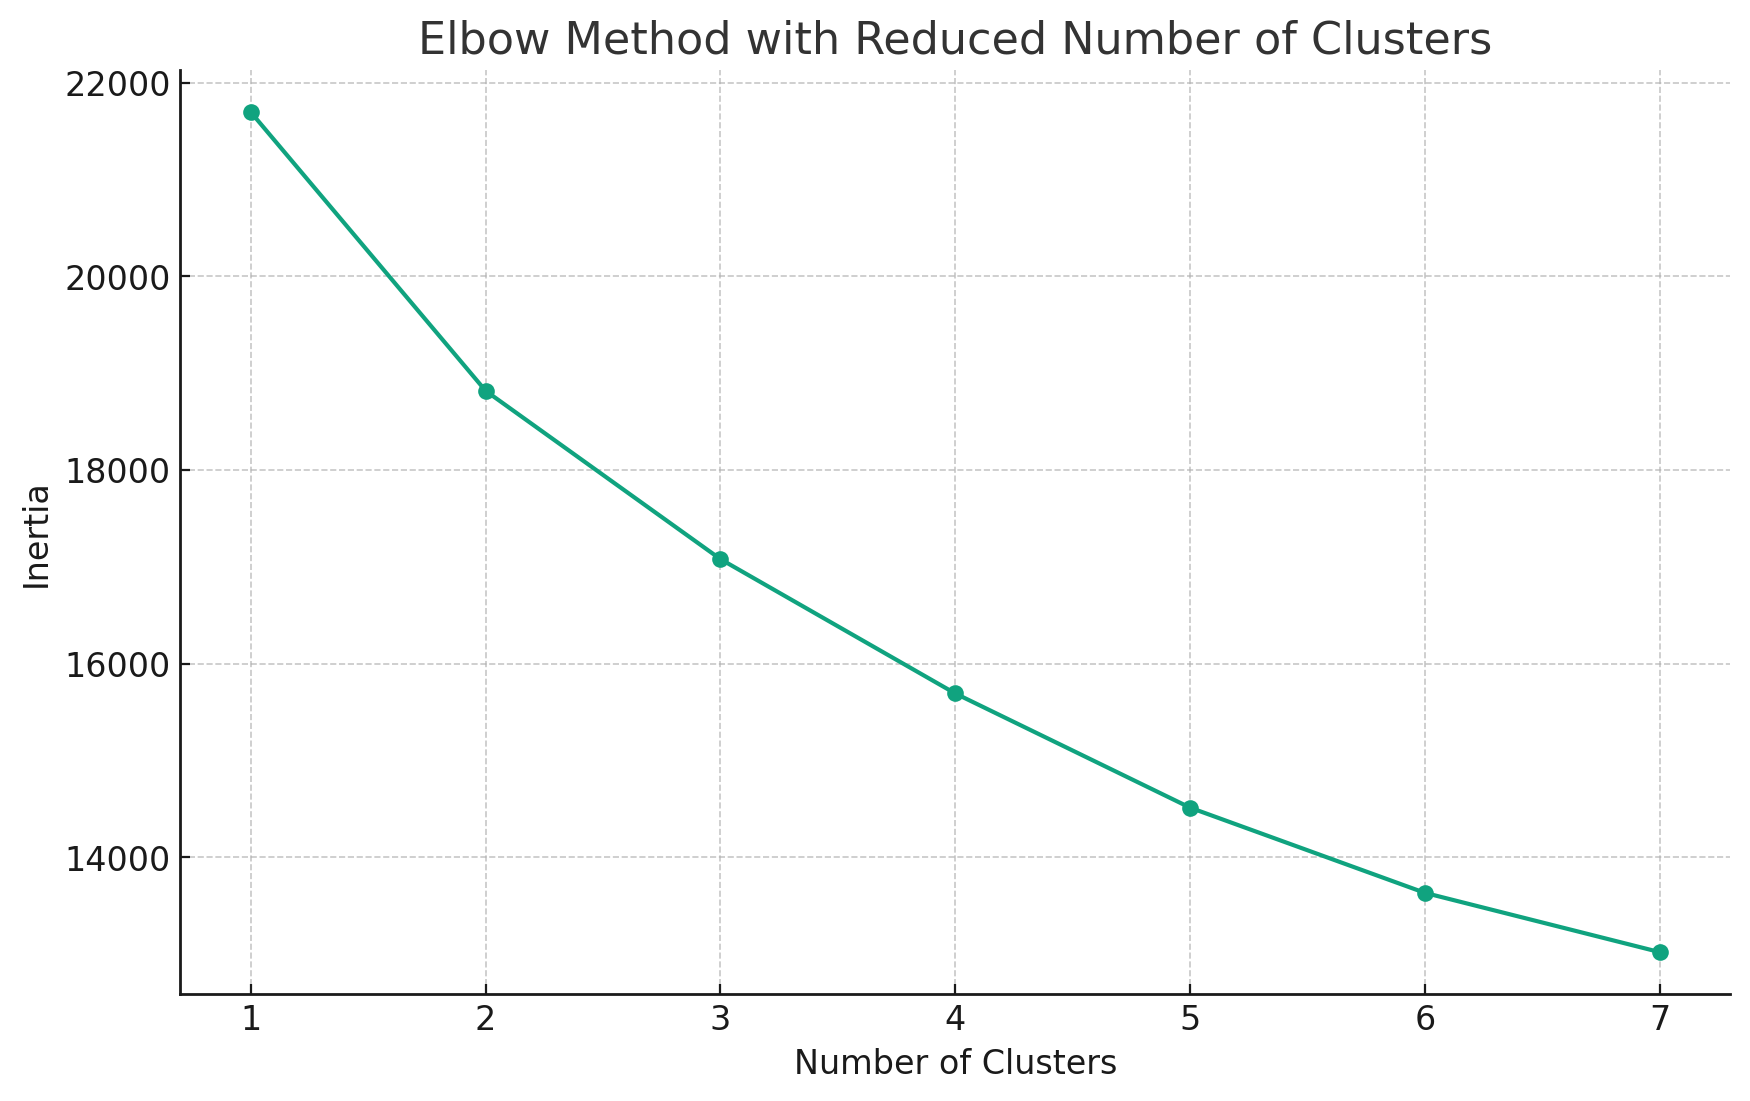
\includegraphics[width=0.9\linewidth]{images/wss.jpg}
  \end{minipage}
  \caption{Within-Cluster Sum of Squares}
  \label{fig:wss}
\end{figure}

Como podemos ver na figura\ref{fig:wss}, o número de agrupamentos deveria ser 6, porque é o ponto de inflexão do gráfico da WSS.

\subsection{Metodologia de Agrupamento}

Voltando à ferramenta de análise de agrupamentos, foi utilizado o algoritmo K-Means \cite{kmeans}, com 6 agrupamentos. Este algoritmo foi escolhido porque é um algoritmo de agrupamento bastante utilizado, e porque é um algoritmo de agrupamento bastante simples, o que é importante para este trabalho.

\subsection{Análise dos Agrupamentos}

Quando o K-Means \cite{kmeans} foi executado, foram criados 6 agrupamentos, e estes agrupamentos foram analisados. Os agrupamentos estão dispostos na tabela\ref{tab:clusters}.

\begin{table}[hbt!]
  \centering
  \begin{tabular}{l c c c c c c c c}
  \toprule
  Cluster & Idade   & Altura     & Peso       & FCVC     & NCP     & CH2O     & FAF     & TUE  \\
  \midrule
  0       & 21.58   & 1.62       & 69.54      & 2.38     & 1.16    & 1.91     & 0.66    & 0.68 \\
  1       & 36.80   & 1.67       & 85.10      & 2.42     & 2.53    & 1.78     & 0.95    & 0.23 \\
  2       & 20.61   & 1.65       & 63.77      & 2.23     & 3.09    & 1.68     & 0.87    & 0.82 \\
  3       & 25.30   & 1.80       & 106.95     & 2.17     & 2.77    & 2.13     & 0.84    & 0.62 \\
  4       & 20.75   & 1.76       & 73.29      & 2.45     & 3.10    & 2.37     & 2.14    & 0.88 \\
  5       & 23.46   & 1.69       & 119.69     & 2.99     & 3.00    & 2.22     & 0.67    & 0.61 \\
  \bottomrule
  \end{tabular}
  \caption{Características dos Agrupamentos}
  \label{tab:clusters}
\end{table}

Como podemos ver na tabela\ref{tab:clusters}, os agrupamentos são bastante diferentes entre si, e cada agrupamento tem características diferentes. Por exemplo, o agrupamento 5 tem uma média de idade de 23.46 anos, uma média de altura de 1.69 metros, uma média de peso de 119.69 quilogramas, uma média de frequência de consumo de vegetais de 2.99, uma média de número de refeições principais de 3.00, uma média de consumo de água diário de 2.22 litros, uma média de frequência de atividade física de 0.67 vezes por semana, e uma média de tempo de uso de dispositivos eletrónicos de 0.61 horas por dia.

\subsection{Estereótipos e Implicações dos Agrupamentos}

Foi despertada a ideia de se criar pessoas virtuais (ou imaginárias), chamadas de \textit{estereótipos}, que representam cada agrupamento. Estes \textit{estereótipos} são pessoas hipotéticas que representam cada agrupamento, e que podem ser utilizadas para entender cada situação. Os \textit{estereótipos} estão dispostos na tabela\ref{tab:stereotypes}.

\begin{table}[hbt!]
  \centering
  \begin{tabular}{p{0.1\linewidth} p{0.2\linewidth} p{0.2\linewidth} p{0.2\linewidth} p{0.2\linewidth}}
  \toprule
  Cluster & Nome & Características & Implicações na Saúde & Influências \\
  \midrule
  0 & Jovem Moderado & Jovem, peso moderado & Peso saudável & Dieta, atividade física e uso de tecnologia moderados. \\
  1 & Mais Velho Tecnológico & Mais velho, peso moderado, baixo uso de tecnologia & Boa saúde, alterações metabólicas possíveis & Dieta saudável, atividade física moderada. \\
  2 & Jovem Ativo & Jovem, peso baixo, mais refeições, ativo & Saudável, metabolismo rápido & Alta atividade física, uso de tecnologia. \\
  3 & Alto Pesado & Alto, pesado & Peso alto, IMC compensado pela altura & Dieta e atividade física moderadas. \\
  4 & Entusiasta do Fitness & Jovem, peso moderado, atividade física alta & Muito saudável & Dieta saudável, alta atividade física. \\
  5 & Indivíduo de Alto Peso & Peso alto & Risco de obesidade & Dieta rica, atividade física moderada. \\
  \bottomrule
  \end{tabular}
  \caption{Resumo das Características dos Agrupamentos}
  \label{tab:stereotypes}
\end{table}

Ao analisar os \textit{estereótipos}, podemos ver que o agrupamento 0 é um jovem moderado, que tem um peso moderado, e que tem uma dieta, atividade física e uso de tecnologia moderados. O agrupamento 1 é um indivíduo mais velho, que tem um peso moderado, e que tem uma dieta saudável, atividade física moderada e baixo uso de tecnologia. O agrupamento 2 é um jovem ativo, que tem um peso baixo, que tem mais refeições, e que tem uma dieta saudável, atividade física alta e uso de tecnologia. O agrupamento 3 é um indivíduo alto e pesado, que tem um peso alto, que tem um IMC compensado pela altura, e que tem uma dieta e atividade física moderadas. O agrupamento 4 é um entusiasta do fitness, que tem um peso moderado, que tem uma atividade física alta, e que tem uma dieta saudável e alta atividade física. O agrupamento 5 é um indivíduo de alto peso, que tem um peso alto, que tem um risco de obesidade, e que tem uma dieta rica e atividade física moderada.

\section{Visualização de Dados}

Para chegar a conclusões mais profundas sobre o conjunto de dados, foi realizada uma visualização de dados, com o objetivo de retirar conclusões sobre a obesidade e a sua relação com os dados demográficos e de estilo de vida. Para a realização desta visualização de dados, foi feito de novo um \textit{detour} para gerar imagens que fossem facilmente exportáveis para o relatório, e que fossem facilmente interpretáveis.

\subsection{Análise de Agrupamentos}

Aqui coloca-se três imagens, as quais representam a comparação entre os agrupamentos e a dois dos atributos fisicos o mais importante e o menos, o peso e a idade e o atributo de estilo de vida mais importante, a frequência de atividade física.

\begin{figure}[hbt!]
  \centering
  \begin{minipage} % two images side by side
    {\linewidth}
    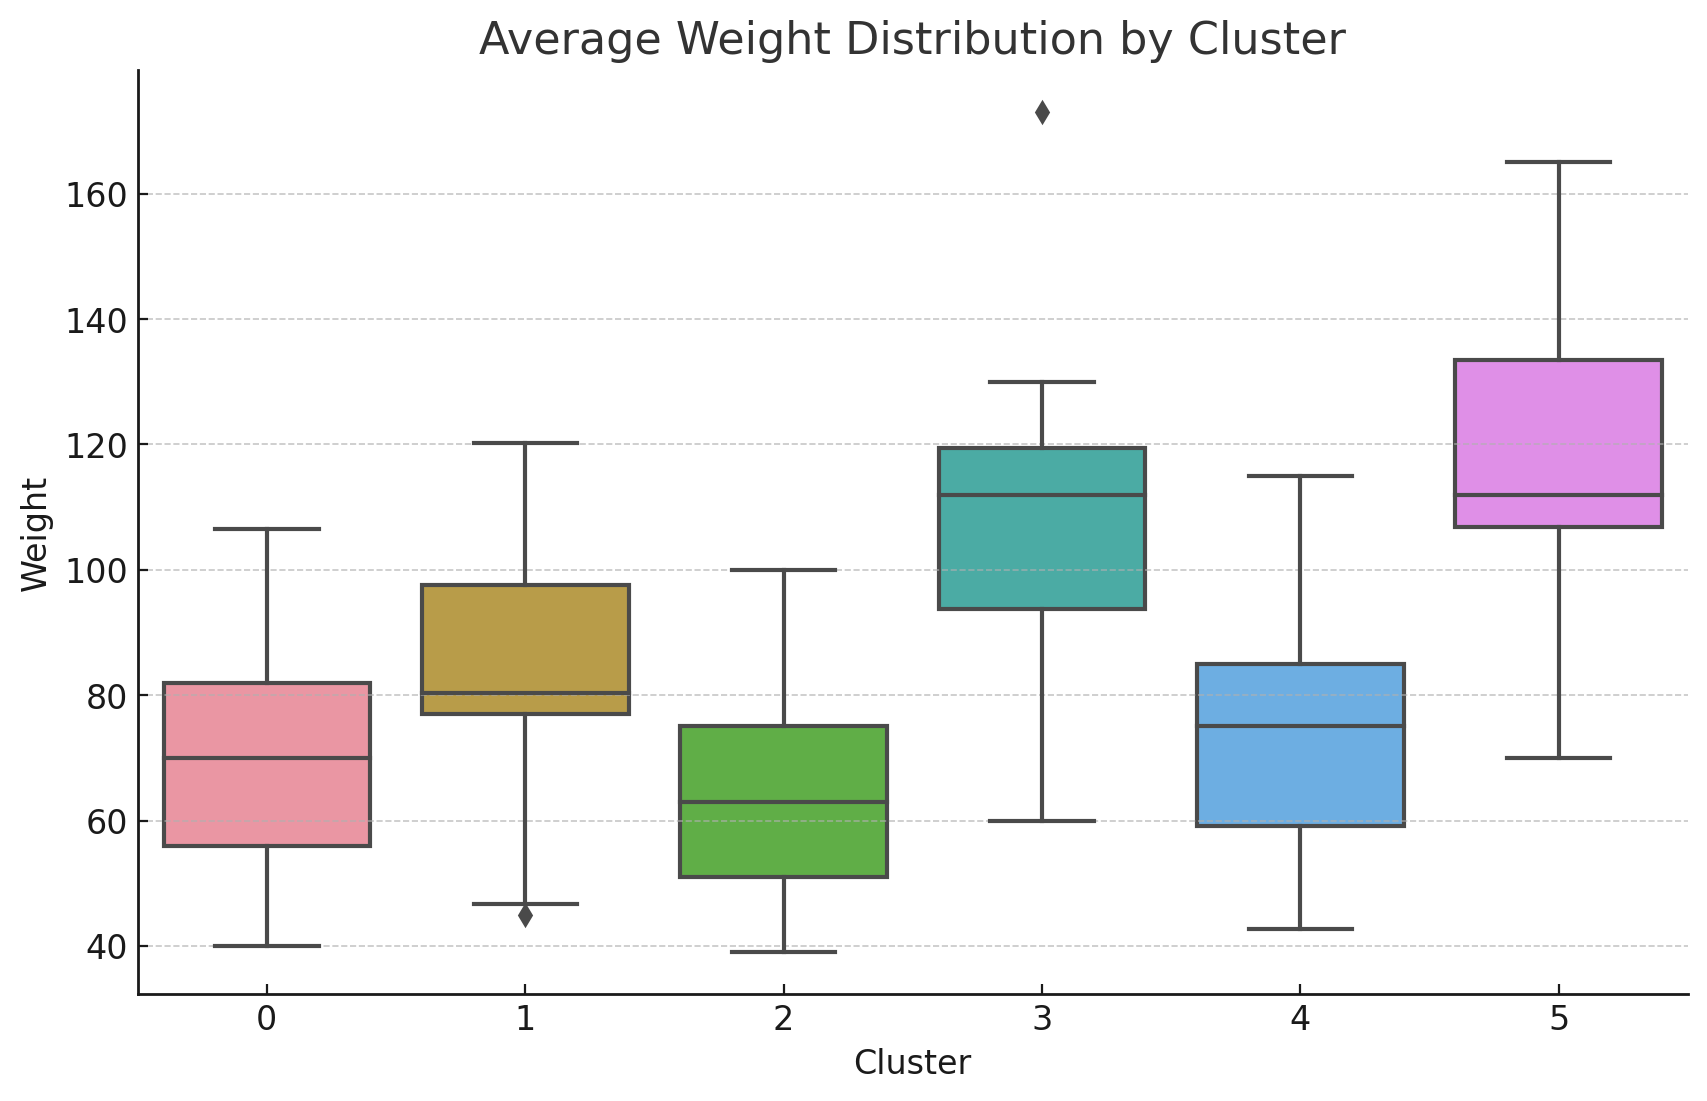
\includegraphics[width=0.45\linewidth]{images/cluster-weight.jpg}
    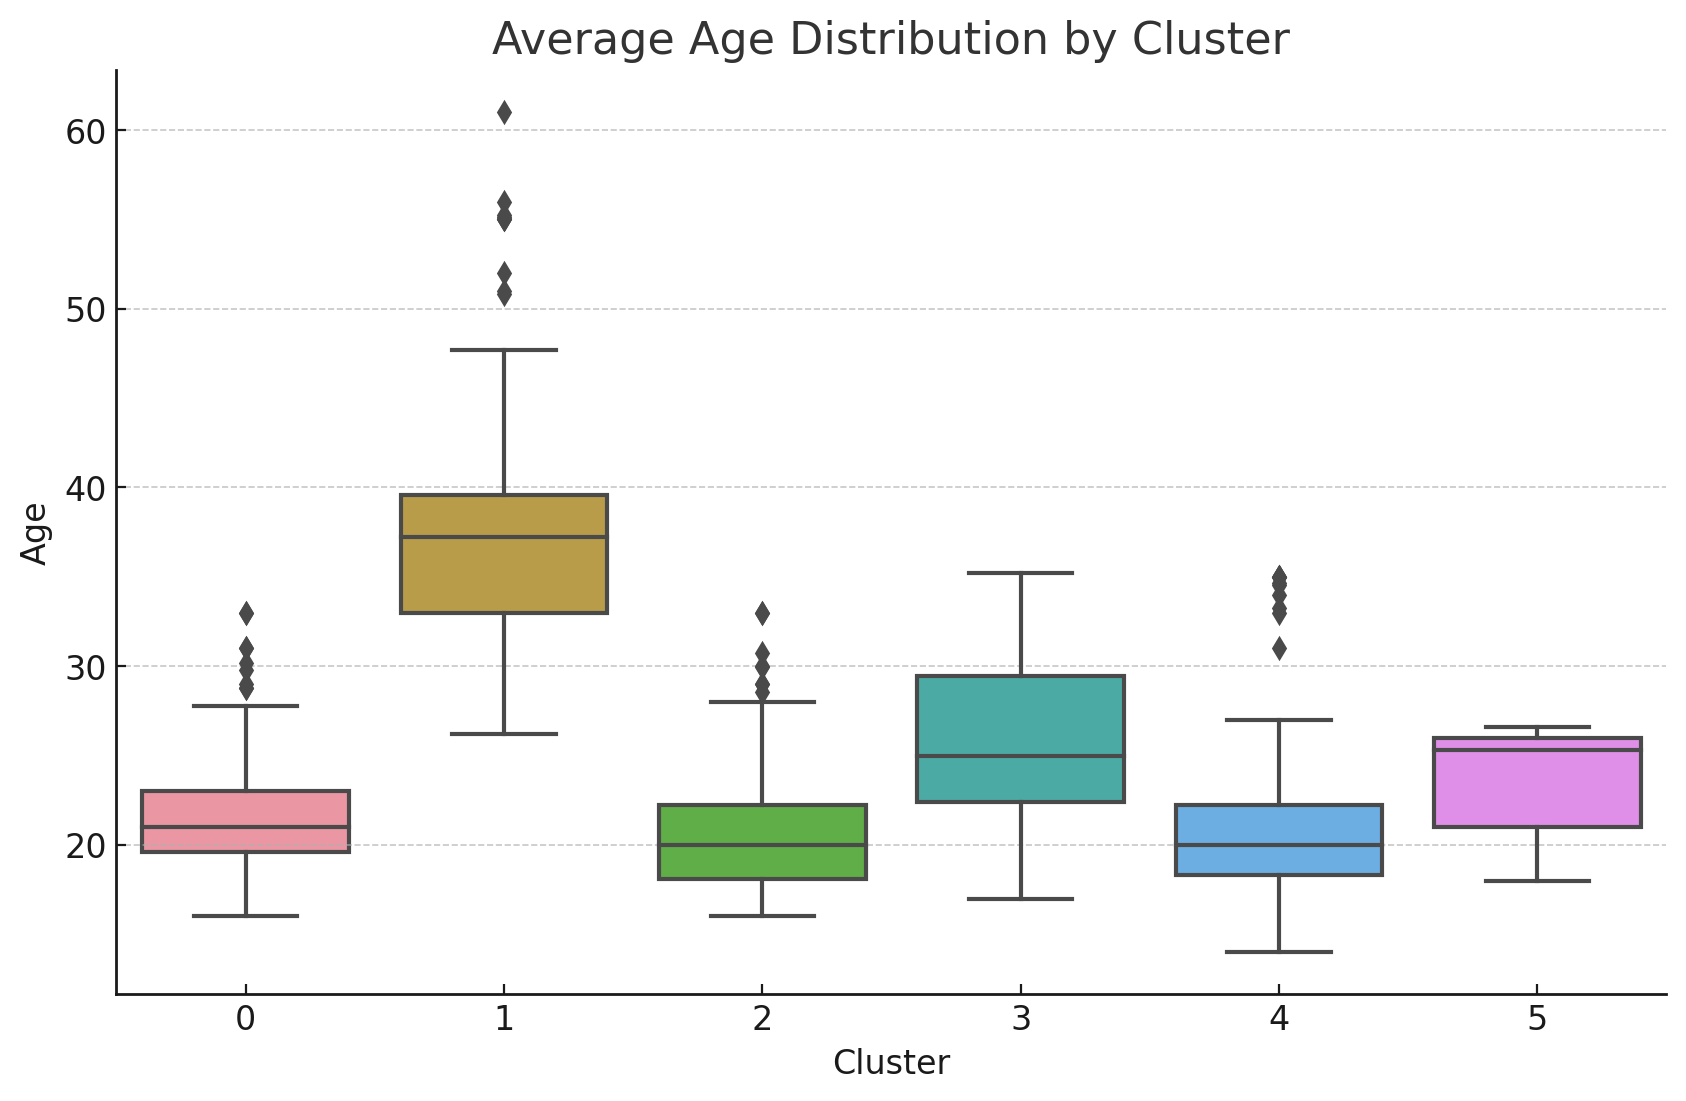
\includegraphics[width=0.45\linewidth]{images/cluster-age.jpg}
  \end{minipage}
  \caption{Comparação entre os Agrupamentos e o Peso e a Idade}
  \label{fig:cluster-weight-age}

  \centering
  \begin{minipage}
    {\linewidth}
    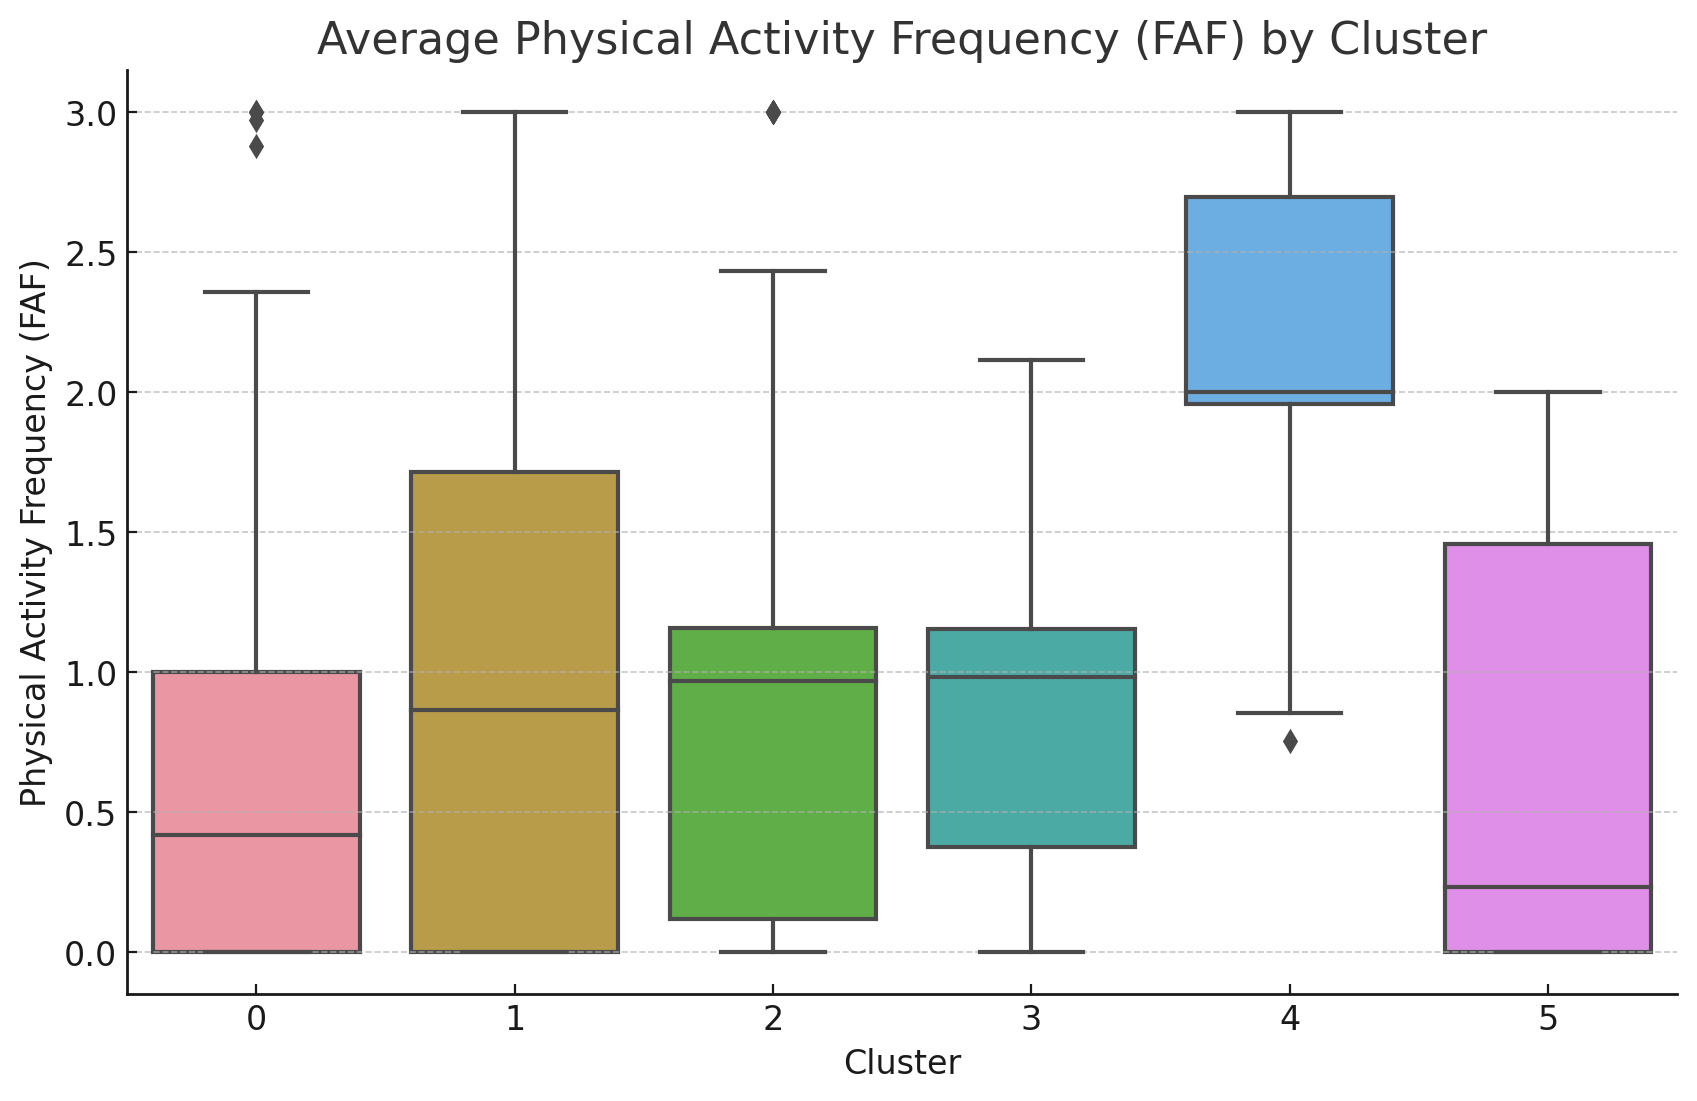
\includegraphics[width=0.9\linewidth]{images/cluster-faf.jpg}
  \end{minipage}
  \caption{Comparação entre os Agrupamentos e a Frequência de Atividade Física}
  \label{fig:cluster-faf}
\end{figure}

Aqui também se coloca o \textit{heatmap} das correlações entre os atributos do conjunto de dados.

\begin{figure}[hbt!]
  \centering
  \begin{minipage}
    {\linewidth}
    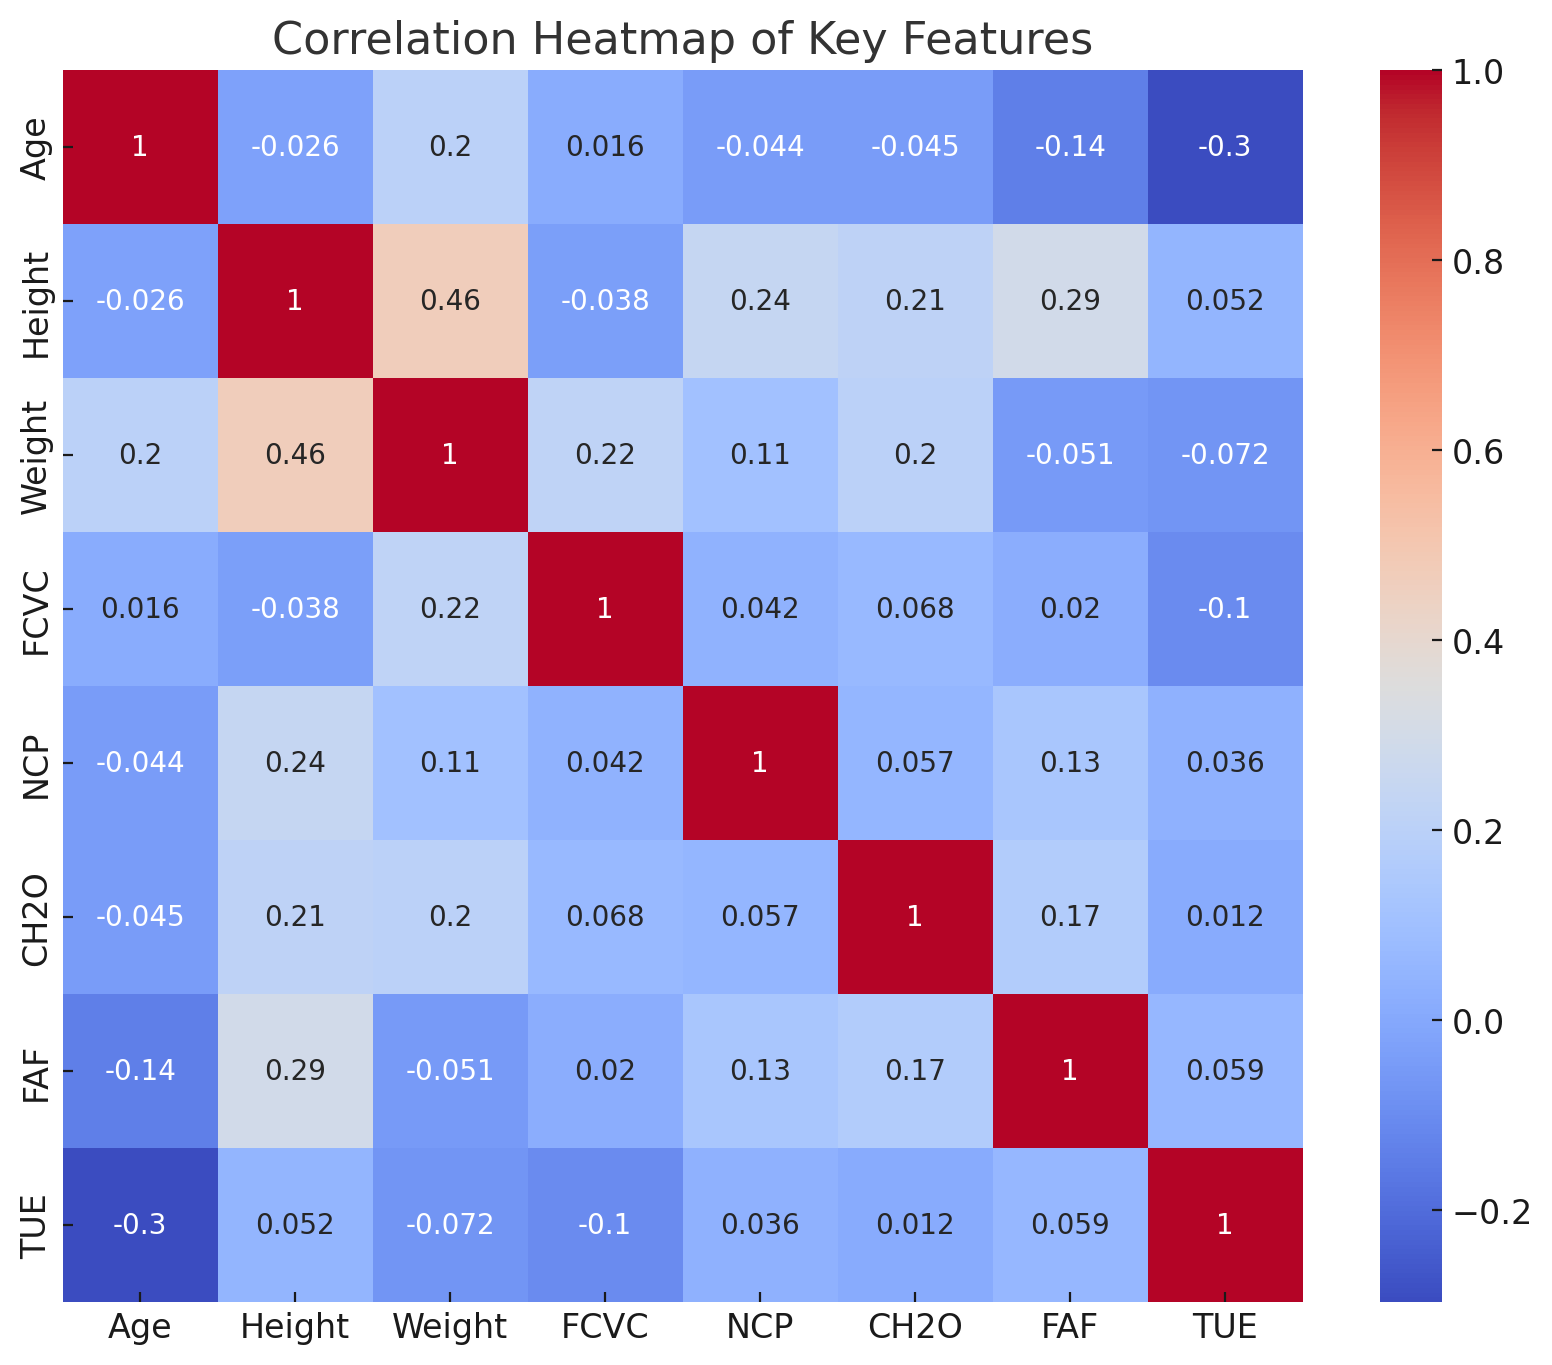
\includegraphics[width=0.9\linewidth]{images/heatmap.jpg}
  \end{minipage}
  \caption{Heatmap das Correlações entre os Atributos}
  \label{fig:correlation-heatmap}
\end{figure}

\subsection{Percepções das Visualizações}

Como podemos ver na figura\ref{fig:cluster-weight-age}, entre os estereótipos, os factores fisicos estão mais concentrados, e o factores de estilo de vida é mais variavel. Com isto podemos ver que os factores fisicos são mais importantes para a obesidade que os factores de estilo de vida.

O mesmo se pode confirmar com o \textit{heatmap} das correlações entre os atributos, que está disposto na figura\ref{fig:correlation-heatmap}. Como podemos ver na figura\ref{fig:correlation-heatmap}, os atributos fisicos têm uma correlação mais forte com a obesidade que os atributos de estilo de vida.

\subsubsection{Resumo das Principais Conclusões}

Em suma podemos concluir que os atributos fisicos são mais importantes para a obesidade que os atributos de estilo de vida, e que os atributos fisicos têm uma correlação mais forte com a obesidade que os atributos de estilo de vida. No entanto, os atributos de estilo de vida também são importantes para a obesidade, e têm uma correlação forte com a obesidade e a idade é o atributo menos importante para a obesidade.

\section{Discussão}
\subsection{Interpretação dos Resultados}

Com todos estes dados podemos afirmar que é importante ter um estilo de vida saudável, e ter um peso saudável. O que pode levar ao ganho de peso pode não ser super-controlavel, mas o que se pode controlar é o estilo de vida, e isso pode atenuar os ganhos de peso. No entanto, infelizmente, o que se pode controlar é não ó o menos importante mas como também o mais dispendioso de tempo, o ser sedentário. Este ponto é o mais importante (dos factores de estilo de vida) pois é o que mais influencia o ganho de peso, e é o que mais influencia a obesidade. Mas infelizmente o mais dificil, sendo que vivemos numa das eras mais sedentárias da história da humanidade, onde o uso de tecnologia é cada vez mais comum, e onde o uso de tecnologia é cada vez mais necessário. Estranhamente o uso da tecnologia não influencia o ganho de peso, mas sim o estilo de vida sedentário, que é o que mais influencia o ganho de peso. Com isto podemos dizer que estar sentado a ver televisão é pior que estar sentado a usar o computador, o que é estranho pois o uso do computador é mais sedentário que o uso da televisão. E suma: mexam-se.

\subsection{Comparação com a Literatura Existente}

Isto vai de acordo com a literatura existente, que diz que o estilo de vida é importante para a obesidade, é importante comer de forma saudável, e é importante fazer atividade física. No entanto, a literatura existente diz que o uso de tecnologia é algo que influencia o sedentarismo, e que influencia o ganho de peso, o que não é o caso deste conjunto de dados. Ou seja, a preguiça não é influenciada pelo uso de tecnologia.


\section{Conclusões e Trabalho Futuro}

Neste trabalho foi feita uma análise de agrupamentos e uma visualização de dados, como tambem modelos de classificação.

\subsection{Resumo dos Resultados}

Concluimos que os atributos fisicos são mais importantes para a obesidade que os atributos de estilo de vida, e que os atributos fisicos têm uma correlação mais forte com a obesidade que os atributos de estilo de vida. No entanto, os atributos de estilo de vida também são importantes para a obesidade, e têm uma correlação forte com a obesidade.

\subsection{Recomendações para Pesquisas Futuras}

Deixo aqui algumas recomendações para pesquisas futuras:

\begin{itemize}
  \item Fazer uma análise de agrupamentos com diferentes algoritmos de agrupamento e com diferentes números de agrupamentos.
  \item Fazer uma análise com novos atributos e remover atributos que não sejam importantes ou que sejam parte do novos atributos agregados (como o IMC).
  \item Rever este mesmo trabalho com novos dados, e com novos modelos de aprendizagem de máquina.
  \item Rever este trabalho e outros da minha autoria, pois tenho notados uma tendência para as Florestas Aleatórias terem um desempenho melhor que os outros modelos de aprendizagem de máquina. Pode ser que seja um problema com a minha implementação, ou um acaso.
\end{itemize}

\bibliographystyle{plain}
\bibliography{easychair}

\end{document}
